\documentclass[a4paper, 12pt]{article}
\usepackage[slovene]{babel}
\usepackage[utf8]{inputenc}
\usepackage[T1]{fontenc}
\usepackage{mathtools}
\usepackage{amsmath}
\usepackage{tikz}
\usepackage{pgfplots}
\usepackage{hyperref}

\setlength{\parindent}{0px}
\setlength{\parskip}{10px}

\begin{document}

	\section*{Linearna regresija}
	\paragraph{}
	Predstavljajmo si, da izvajamo fizikalni poskus. Imamo vzmet, na kateri merimo raztezek v odvisnosti od sile, s katero napenjamo vzmet (na vzmet obešamo uteži z znano težo in merimo raztezek).

	\paragraph{}
	Velja Hookov zakon, $F = k x$, torej sta $x$ in $F$ med seboj linearno odvisna. Poskušali bomo najti premico, ki se bo najbolje prilegala danim točkam v ravnini.

	\paragraph{}
	Če imamo 2 točki $T_1(x_1, y_1), T_2(x_2, y_2)$, lahko brez težav najdemo premico, ki gre točno skozi niju. Če pa je točk več, ni nujno, da obstaja premica, ki gre skozi vse točke. Lahko bi našli polinom, ki se natančno prilega vsem točkam, vendar to v primeru linearne odvisnosti ni dobra ideja, saj bi bila krivulja natančna samo v tistih točkah, drugje pa bi bila odstopanja velika.
	Iščemo taka $a$ in $b$, da se bo premica kar najbolje prilegala danim točkam. Če gre premica skozi neko točko $T_i(x_i, y_i)$, potem velja:

	$$0 = a x_i + b - y_i$$

	Ker pa naša premica ne poteka direktno skozi vse točke, pride do napake, ki jo bomo v točki $T_i$ označili z $\varepsilon_i$.

	$$\varepsilon_i = a x_i + b - y_i$$

	\paragraph{}
	Napaka je lahko pozitivna ali negativna, odvisno ali točka leži pod ali nad premico. Želimo zmanjšati velikost vseh napak, ne glede na to, ali so pozitivne ali negativne. (Lahko bi preprosto sešteli absolutne vrednosti napak, ampak pozneje funkcije ne bi mogli odvajati.) Zato seštejemo kvadrate vseh napak.

	$$\varepsilon = \sum_{i=1}^{N} \varepsilon_i^2$$
	$$\varepsilon = \sum_{i=1}^{N} (a x_i + b - y_i)^2$$

	\paragraph{}
	Naš cilj je, da minimiziramo to napako. To bomo naredili s pomo"cjo gradientnega spusta.

	\section*{Gradientni spust}
	\paragraph{}
Z gradientnim spustom i"s"cemo minimum ali pa maksimum neke funkcije, to pomeni kje ima funkcija najve"cjo oziroma najmanj"so vrednost. Gradientni spust je zelo primitivna metoda kjer se preprosto premikamo v smer kamor funkcija nara"s"ca oziroma pada.

\paragraph{}
To si lahko predstavljamo s pomo"cjo slepega "cloveka, ki "zeli priti na vrh Golovca. Ko bo na"s "clovek, poimenujmo ga Lojze, na neki to"cki hriba, ne bo videl v katero smer mora hoditi (ker je slep), "cutil pa bo kako strm je hrib. Na za"cetku, ko je hrib bolj strm, bo Lojze naredil ve"cji korak, ko pa se bo pribli"zeval vrhu in bo hrib postajal manj strm, pa bo delal manj"se korake, ker se lahko druga"ce zgodi, da bo prestopil vrh in se zna"sel na drugi strani Golovca.

\paragraph{}
Z bolj matemati"cnimi besedami: gradient nam pove smer naraščanja funkcije. Preden nadaljujemo z gradientom, moramo definirati kaj nam predstavlaj strmino funkcije (nara"s"canje in padanje). To bomo naredili z odvodi.

\subsection*{Odvod}
\paragraph{}
Kot smo "ze omenili, nam gradient predstavlja strmino funkcije. Preden se lahko naprej pogovarjamo o gradientnem spust, potrebujemo definirati strmino funkcije.

\paragraph{}
Odvod neke funkcije $f(x)$ je strmina te funkcije v to"cki $x$. Odvod je pozitiven "ce funkcija nara"sca in negativen "ce funkcija pada. Ve"cji kot je odvod, bolj strma je funkcija v dani to"cki. Odvod funkcije $f(x)$, ki ga ozna"cimo z $f'(x)$, nam torej pove, kakšen je koeficient tangente na graf fukncije $ f(x) $ v točki $x$.


\begin{figure}[!h]
	\centering
	\caption{Odvod}
	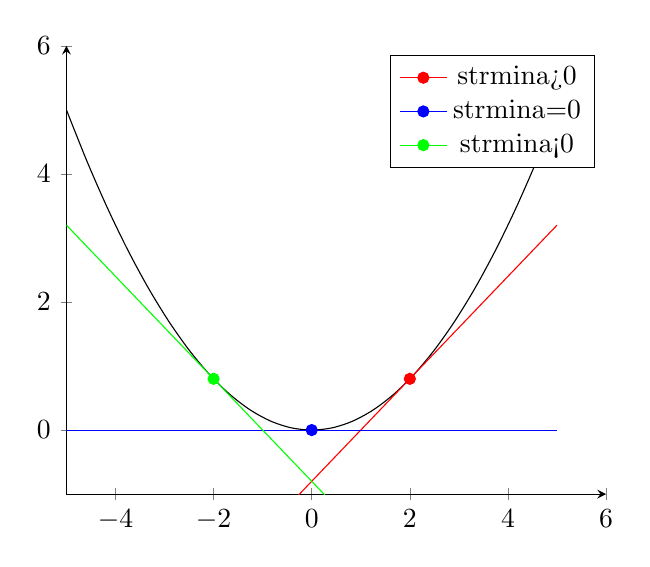
\begin{tikzpicture}
	\begin{axis}[axis lines=left, xmin=-5, xmax=6, ymin=-1, ymax=6]
	\addplot[color=black, smooth]{0.2*x^2};

	\addplot[color=red]{0.8*x - 0.8};
	\addplot[color=red, mark=*] coordinates {(2, 0.8)};

	\addplot[color=blue]{0};
	\addplot[color=blue, mark=*] coordinates {(0, 0)};

	\addplot[color=green]{-0.8*x - 0.8};
	\addplot[color=green, mark=*] coordinates {(-2, 0.8)};
	\legend{,,strmina>0,,strmina=0,,strmina<0}
	\end{axis}
	\end{tikzpicture}
\end{figure}


\subsection*{Delni odvod}
\paragraph{}
Pri funkciji, ki je odvisna od ve"cih parametrov se zakomplicira tudi odvod. Tako funkcijo moramo odvajati po vsaki spremenljivki posebej, kar pomeni da potrebujemo funkcijo $f(x,y)$ odvajati po $x$ in po $y$. S tem dobimo dva odvoda. Odvod po $x$ nam pove kako funkcija nara"s"ca oziroma po $x$ osi, odvod po $y$ pa nam seveda pove kako funkcija nara"s"ca oziroma pada po $y$ osi. Takemu odvodu re"cemo delni odvod, zapi"semo pa ga kot $\frac{\partial f(x,y)}{\partial x}$ za delni odvod po $x$ in $\frac{\partial f(x,y)}{\partial y}$ za delni odvod po $y$.

\paragraph{}
Za trenutek se vrnimo na za"cetni problem, ki nas je pripeljal do sem. "Zelelimo najti tako premico, ki se najbolj prilega vsem danim to"ckam. Definirali smo "ze skupno napako in ugotovili da je na"sa napaka funkcija, ki je odvisna od spremenjivk $a$ in $b$. Sedaj lahko pora"cunamo, kako strma je na"sa napaka za dani $a$ in $b$ po parametru $a$ in kako strma je po parametru $b$. Druga"ce povedano, izra"cunamo lahko delni odvod napake po $a$ in delni odvod napake po $b$.
$$\frac{\partial \varepsilon}{\partial a} =
\sum_{i=1}^{N} 2 \frac{\partial (a x_i + b - y_i)}{\partial a} =
2 \sum_{i=1}^{N} (a x_i + b - y_i)x_i$$

$$\frac{\partial \varepsilon}{\partial b} =
\sum_{i=1}^{N} 2 \frac{\partial (a x_i + b - y_i)}{\partial b} =
2 \sum_{i=1}^{N} (a x_i + b - y_i)\cdot1 = 2 \sum_{i=1}^{N} (a x_i + b - y_i)$$

\subsection*{Gradient}
\paragraph{}
Gradient neke funkcije je vektor, ki ka"ze v smer nara"s"canja te funkcije. Gradient funkcije $f$ ozna"cimo z $\nabla f$. Pri funkciji z enim parametrom ($f(x)$), ima gradient te funkcije samo eno komponento, to je odvod funkcije $f(x)$. To zapi"semo kot:
\[\nabla f = \begin{pmatrix}f'\end{pmatrix} \]

\paragraph{}
"Ce je funkcija odvisna od dveh spremenljivk, je vsaka komponenta gradienta en delni odvod. To pomeni, da nam prva komponenta gradienta pove kam nara"s"ca funkcija in kako strma je glede na prvi parameter, druga komponenta gradienta pa nam pove kam nara"s"ca funkcija in kako strma je glede na drugi parameter funkcije.

\paragraph{}
Za la"zjo predstavo si oglejmo gradient funkcije $f(x,y)$. Prva komponenta tega gradienta nam bo povedala strmino funkcije v smeri $x$ osi, druga komponenta tega gradienta pa nam pove strmino funkcije v smeri $y$ osi.

\paragraph{}
V splo"snem lahko gradient funkcije $f$, ki je odvisna od $n$ parametrov zapi"semo kot:
\[\nabla f = \begin{pmatrix}
\frac{\partial f}{\partial x_1} &
\frac{\partial f}{\partial x_2} &
\frac{\partial f}{\partial x_2} &
\dots &
\frac{\partial f}{\partial x_n}
\end{pmatrix} \]

Gradient na"se napake bi izgledal takole:
\[\nabla \varepsilon = \begin{pmatrix}
\frac{\partial \varepsilon}{\partial a} &
\frac{\partial \varepsilon}{\partial b}
\end{pmatrix} \]
	
	\section*{Prilagajanje premice}
	\paragraph{}
Sedaj ko razumemo kaj je gradient, se lahko vrnemo na na"s za"cetni problem, to je najti tako premico, ki se najbolj prilega $N$ to"ckam. Na tem primeru bomo razlo"zili tudi gradientni spust.

\paragraph{}
Najprej se spomnimo, kaj sploh "zelimo narediti. Na"sa funkcija je $\varepsilon_i = ~ax_i + ~b - ~y_i$ kjer $\varepsilon_i$ predstavlja napako te funkcije v to"cki $T_i(x_i, y_i)$. Skupno napako smo definirali kot: $\varepsilon = \sum_{i=1}^{N} \varepsilon_i^2$ in jo tudi odvajali. Definirali smo tudi gradient na"se funkcije.


\paragraph{}
Za"cetna parametra $a$ in $b$ dolo"cimo sami, kasneje pa jih spreminjamo z matemati"cnimi ena"cbami. Od za"cetnih parametrov je odvisna natan"cnost na"sega rezultata. Ve"c o tem bomo povedali kasneje.

\paragraph{}
Vemo torej, v katero smer na"sa funkcija napake nara"s"ca. Sedaj se lahko premaknemo v nasprotno smer, to pomeni tja, kamor na"sa funkcija pada. To da se premaknemo v neko smer, pomeni da spremenimo na"s $a$ in $b$ tako, da bo napaka manj"sa. Parameter $a$ zmanj"samo za vrednost prve komponente na"sega gradienta, ker je ta komponenta delni odvod napake po $a$ in nam pove, kako se napaka spreminja, "ce spreminjamo $a$. Parameter $b$ pa seveda zmanj"samo za vrednost druge komponente na"sega gradienta.

Pa razpi"simo te spremembe. Spremembo $a$ lahko napi"semo kot:
\[\Delta a = -(\nabla \varepsilon)_1 \cdot \lambda\]
Minus uporabimo zato, ker se premikamo v smer kamor funkcija pada, to pomeni nasprotno od tega kamor ka"ze gradient. $\lambda$ je konstanta, ki nam predstavlja kako hitro spreminjamo na"s parameter. $\lambda$ dolo"cimo mi. O to"cnem pomenu $\lambda$ se bomo pogovorli nekoliko kasneje.

Spremembo $b$ pa lahko zapi"semo kot:
\[\Delta b = -(\nabla \varepsilon)_2 \cdot \lambda\]

\paragraph{}
V te dve ena"cbi lahko sedaj vstavimo delna odvoda, ki smo ju nara"cunali prej in dobimo:
\[\Delta a = -\sum_{i=1}^{N} (a x_i + b - y_i)x_i \cdot \lambda \]
\[\Delta b = -\sum_{i=1}^{N} (a x_i + b - y_i) \cdot \lambda \]

Pri obeh ena"cbah smo se lahko znebili $2$, ker lahko pove"camo na"so konstanto $\lambda$ in dobimo enak rezultat.

\paragraph{}
Sedaj ko vemo za koliko moramo spremeniti na"sa parametra $a$ in $b$, jih seveda tudi spremenimo. Na"sa nova parametra sta torej:
\[a = a + \Delta a \]
\[b = b + \Delta b \]

\paragraph{}
Z vsem tem delom smo en korak bli"zje na"sim "zelenim vrednostim. Ta postopek moramo ponoviti "se velikokrat, zato izkoristimo ra"cunalnik. Ve"ckrat kot ponovimo postopek, bolj natan"cen bo na"s rezultat. Temu spreminjanju parametrov v smer gradienta pravimo gradientni spust.

\paragraph{}
Natančnost našega rezultata je odvisna od $\lambda$ (velikost premika) in začetnih vrednost spremenljivk $a$ in $b$. Z manjšo velikostjo premika bo rezultat bolj natančen, vendar bomo morali postopek večkrat ponoviti. Ker s postopkom isčemo samo lokalne minimume, nam začetna vrednost spremenljivk določi kateri minimum bomo našli.

	\section*{Linerana regresija elipse}
	\paragraph{}
Seveda se nam ni treba omejiti samo na prilagajanje premice to"ckam. "Ce imamo na primer to"cke na kro"znici nekega planeta, bomo tem to"ckam prilagodili elipso. Recimo da imamo $N$ točk krožnice nekega planeta $T_i(x_i, y_i)$.~\footnote{To"cke za planete so podane v eklipti"cnem koordinatnem sistemu. Ve"c si lahko preberete v \hyperref[eklipticni_sistem]{dodatku}.} Podobno kot pri prej"snjem primeru, bomo tudi tokrat iskali funkcijo, ki se to"ckam najbolj prilega. Tokrat bomo namesto premice iskali elipso, saj se elipsa bolj prilega kro"znici planeta kot premica.

\paragraph{}
Ker je elipsa sto"znica bomo za funkcijo, ki jo prilagajamo vzeli splo"sno ena"cbo sto"znic:
$$Ax^2 + Bxy + Cy^2 + Dx + Ey + F = 0$$

Tako kot prej se nam bo pojavila napaka, ki jo ozna"cimo z $\varepsilon$.
$$\varepsilon_i = Ax_i^2 + Bx_iy_i + Cy_i^2 + Dx_i + Ey_i + F$$

\paragraph{}
Za razliko od premice je oblika sto"znice odvisna od "sestih parametrov namesto dveh. To so: $A, B, C, D, E$ in $F$. Zato bomo spreminjali teh "sest parametrov. To pomeni, da je na"sa napaka funkcija, ki je odvisna od "sestih parametrov.

\paragraph{}
Podobno kot pri premici najprej definiramo skupno napako kot vsoto kvadratov vseh napak:
\[\varepsilon = \sum_{i=1}^{N}\varepsilon_i^2\]
\[\varepsilon = \sum_{i=1}^{N} (Ax_i^2 + Bx_iy_i + Cy_i^2 + Dx_i + Ey_i + F)^2\]

\paragraph{}
Enako kot pri premici moramo na"so napako parcialno odvajati po spremenjivkah, od katerih je na"sa napaka odvisna. To pomeni, da moramo izra"cunati parcialni odvod napake po $A, B, C, D, E$ in $F$. Parcialni odvodi za ena"cbo sto"znic so:
$$\frac{\partial \varepsilon}{\partial A} = \sum_{i=1}^{N}2(Ax_i^2 + Bx_iy_i + Cy_i^2 + Dx_i + Ey_i + F)(x_i^2)$$
$$\frac{\partial \varepsilon}{\partial B} = \sum_{i=1}^{N}2(Ax_i^2 + Bx_iy_i + Cy_i^2 + Dx_i + Ey_i + F)(x_iy_i)$$
$$\frac{\partial \varepsilon}{\partial C} = \sum_{i=1}^{N}2(Ax_i^2 + Bx_iy_i + Cy_i^2 + Dx_i + Ey_i + F)(y_i^2)$$
$$\frac{\partial \varepsilon}{\partial D} = \sum_{i=1}^{N}2(Ax_i^2 + Bx_iy_i + Cy_i^2 + Dx_i + Ey_i + F)(x_i)$$
$$\frac{\partial \varepsilon}{\partial E} = \sum_{i=1}^{N}2(Ax_i^2 + Bx_iy_i + Cy_i^2 + Dx_i + Ey_i + F)(y_i)$$
$$\frac{\partial \varepsilon}{\partial F} = \sum_{i=1}^{N}2(Ax_i^2 + Bx_iy_i + Cy_i^2 + Dx_i + Ey_i + F)$$

\paragraph{}
Da najdemo najbolj"se parametre, pri katerih bo funkcija imela najmanj"so napako, bomo ponovno uporabili gradientni spust. Za razliko od gradientnega spusti pri eni premici bomo tokrat spreminjali "sest parametrov. Na"s gradient je torej:
$$\nabla \varepsilon = \begin{pmatrix}
\frac{\partial \varepsilon}{\partial A} &
\frac{\partial \varepsilon}{\partial B} &
\frac{\partial \varepsilon}{\partial C} &
\frac{\partial \varepsilon}{\partial D} &
\frac{\partial \varepsilon}{\partial E} &
\frac{\partial \varepsilon}{\partial F}
\end{pmatrix}$$

To pomeni da so na"se spremembe parametrov:
$$\Delta A = -(\nabla \varepsilon)_1 \cdot \lambda$$
$$\Delta B = -(\nabla \varepsilon)_2 \cdot \lambda$$
$$\Delta C = -(\nabla \varepsilon)_3 \cdot \lambda$$
$$\Delta D = -(\nabla \varepsilon)_4 \cdot \lambda$$
$$\Delta E = -(\nabla \varepsilon)_5 \cdot \lambda$$
$$\Delta F = -(\nabla \varepsilon)_6 \cdot \lambda$$

Iz "cesar sledi, da so na"si novi parametri podobno kot pri premici:
$$A = A + \Delta A$$
$$B = B + \Delta B$$
$$C = C + \Delta C$$
$$D = D + \Delta D$$
$$E = E + \Delta E$$
$$F = F + \Delta F$$

\paragraph{}Pravilnost na"sega rezultata je seveda odvisna od: koliko ponovitev bomo naredili, kolik"sna bo na"sa $\lambda$ in kak"sne za"cetne vrednosti $A, B, C, D, E$ in $F$ smo si izbrali.

	
	\section*{Logistična regresija}
	\paragraph{}
Glavna razlika med logistično in linearno regesijo je, da pri linearni regresiji določamo zvezno spremenljivko ($y$ je odvisen od $x$), medtem ko nam pri logistični regresiji model vrne kakšna je verjetnost, da vhodni podatki sodijo v določeno kategorijo.

\paragraph{}
To si lahko predstavljamo kot funkcijo, ki vrne ve"c parametrov. Linearna regresija nam predstavlja funkcijo, ki vrne eno "stevilko oziroma parameter. Logisti"cna regresija pa je funkcija, ki vzame ve"c parametrov in vrne ve"c parametrov, to je "stevilk.

\paragraph{}
Logisti"cna regresija se uporablja za klasifikacijo. Eden izmed takih primerov je prepoznavanje "stevil na sliki. "Ce se lotimo prepoznavanja enomestnih "stevil, bi nam logisti"cna regresija vrnila 10 parametrov oziroma "stevil. Vsako izmed teh "stevil nam predstavlja verjetnost, da je na sliki dolo"cena cifra. Prvo "stevilo nam recimo predstavlja verjetnost, da je na sliki 0, drugo da je na sliki 1, tretje da je na sliki 2 in tako naprej.

	
	\section*{Nevronska mre"za}
	\paragraph{}
Logisti"cno regresijo pa lahko zakompliciramo "se nekoliko bolj. "Stevila, ki nam jih vrne logisti"cna regresija lahko vzamemo kot vhodne parametre na novi logisti"cni regresiji. In potem lahko to ponovimo "se enkrat, dvakrat ali pa celo $n$-krat. Takemu sistemu pravimo nevronska mre"za. 


	\section*{Dodatno}
	\subsection*{Ekliptični koordinatni sistem}
\label{eklipticni_sistem}
	
\paragraph{}
Eklipti"cni koordinatni sistem je eden izmed koordinatnih sistemov za določanje lege nebesnih teles. Lokacijo se dolo"ca glede na sonce. Tako kot imamo za dolo"canje lokacije na zemlji zemljepisno "sirino in zemljepisno dol"zino, imamo pri eklipti"cnem koordinatnem sistemu eklipti"cna dol"zino in eklipti"cno "sirino, ki pomenita isto, samo da namesto to"cke na zemljinem povr"sju definirata to"cko na povr"sju sonca. Predstavljamo si, da smo na Soncu (seveda pono"ci, da ni prevro"ce) in za dolo"canje koordinat z latitudo in longitudo naredimo isto kot na Zemlji, samo da je tokrat Sonce na"sa Zemlja. Za dodatek imamo "se tretji podatek, to je razdalja od Sonca. Da povzamemo:
\begin{description}
	\item[$l$] longtituda, ekliptična dolžina, od $0^\circ$ do $360^\circ$.
	\item[$b$] latituda, ekliptična širina od $-90^\circ$ do $90^\circ$.
	\item[$r$] razdalja
\end{description}

Eklipti"cna "sirina je definirana egoisti"cno, tako da je ravnina na kateri le"zi zemljina orbita, vedno 0º latitude.

Eklipti"cna "sirina je definirana glede na neko son"sno pego.

\paragraph{}
V kartezične koordinate lahko podatke pretvorimo na podoben na"cin kot polarne koordinate pretvarjamo v kartezi"cne. Samo da imamo tokrat neke vrste 3D polarni zapis. Na"se formule so:\newpage
$$x = r \cos b \cos l$$
$$y = r \cos b \sin l$$
$$z = r \sin b$$

\paragraph{}
Te koordinate "zelimo sedaj pretvoriti iz 3D v 2D koordinatni sistem, da jih bomo lahko uporabili v ena"cbi za sto"znice. To bi lahko naredili tako, da bi vzeli projekcijo na"sih to"ck na ravnino. Ker pa tiri ve"cine planetov v na"sem oson"cju ležijo v (skoraj) isti ravnini, se bomo naredili fizike in preprosto zanemarili $z$ koordianto.

\end{document}
